\documentclass{beamer}
\usetheme{CambridgeUS}
\usepackage{amsmath}
\usepackage{amssymb}
\usepackage{tikz}
\usetikzlibrary{arrows.meta, positioning}
\usepackage{cancel}
\usetikzlibrary{positioning}

\tikzset{
box/.style={
draw,
rectangle,
rounded corners,
align=left,
font=\small,
inner sep=4pt,
fill=green!15
}
}



\title{On Solving the Multiple Variable Gapped Longest Common Subsequence Problem}

\author{Marko Djukanović\inst{1,2, 6}  \and Nikola Balaban\inst{2}  \and
Christian Blum\inst{3}  \and 
Aleksandar Kartelj\inst{4}  \and
Sašo Džeroski\inst{5}  \and
Žiga Zebec\inst{6}
}

\institute{ $^1$University of Nova Gorica, Nova Gorica, Slovenia \\ 
$^2$Faculty of Natural Sciences and Mathematics, University of Banja Luka, Banja Luka, Bosnia and Herzegovina \\ 
$^3$Artificial Intelligence Research Institute (IIIA-CSIC), Barcelona, Spain \\ 
$^4$Faculty of Mathematics, University of Belgrade, Belgrade, Serbia \\
$^5$Jožef Stefan Institute, Ljubljana, Slovenia \ \\
$^6$Institute of Information Sciences (IZUM), Maribor, Slovenia \\ \vspace{0.3cm}

\footnotesize{-- \textcolor{blue}{Eurocast 2026: 20th International Conference on Computer Aided Systems Theory, February 23-27, 2026,  Las Palmas de Gran Canaria, Spain}--}
\centering

\includegraphics[width=90pt,height=50pt]{SMASH_CMYK-ENG-horizontal_on_white.pdf}~ \hfill
\includegraphics[width=80pt,height=50pt]{IFEEL\_1.png}~\hfill
\includegraphics[width=110pt,height=40pt]{CofundedbytheEU\_RGB\_NEG.png}
}

\begin{document}
\begin{frame}[plain]
    \maketitle
\end{frame}

\begin{frame}{Outline}
    
    \begin{itemize}
        \item Introduction \& Preliminaries \vspace{0.2cm}
        \item Problem Definition  \vspace{0.2cm}
        \item Graph state space  \vspace{0.2cm}
        \item Iterative multi-source Beam Search  \vspace{0.2cm}
        \item Experimental Evaluation
        \begin{itemize}
            \item General problem
            \item Special problem
        \end{itemize} \vspace{0.2cm}
        \item Conclusions
    \end{itemize}
\end{frame}

\begin{frame}{Introduction}
   \begin{itemize}
       \item Objects we deal with: sequences (strings) over finite alphabet 
       \begin{itemize}
       \item DNA/RNA over $\{\texttt{A}, \texttt{T}, \texttt{G}, \texttt{C/U}\}$
       \item Proteins over 20 (canonical) amino acids: $\{\texttt{A}, \texttt{C}, \texttt{D}, \texttt{E}, \texttt{P}, \texttt{Q} ...\}$ 
       \end{itemize} \vspace{0.3cm}
       \item Computational biology
       \begin{itemize}
          \item \textbf{One of central tasks:} sequence comparison, finding common motifs between sequences
          \item compare structurally but also semantically/functionality 
          \item sequence alignment problems 
       \end{itemize} \vspace{0.4cm}
       
       \item Subsequences: reveal structural similarities $\rightarrow$ \textcolor{blue}{\textbf{Longest commmon subsequence problem}} variants
   \end{itemize}
\end{frame}

\begin{frame}{Longest common subsequence problem (LCSP)}
    
    \begin{itemize}
      \item Basic problem in Computational biology
      \item Intensively solved over last 50 years
      \begin{itemize}
      \item theoretically as well as practically 
      \item Practically: many approximation algorothms, (meta-) heuristics, exact approaches, etc.
      \end{itemize}
    \end{itemize}
    
    \begin{definition}[LCSP]
        \textbf{Input}: Given a set of sequences $S=\{s_1, \ldots, s_m\}$ \\
        \textbf{Task}: Find a   subsequence $s$ which is \textcolor{blue}{common} for all sequences from $S$ of \textcolor{blue}{maximum} possible length. 
    \end{definition}
    \begin{example}
       Input: S=\{\texttt{\textcolor{red}{A}A\textcolor{red}{T}\textcolor{red}{T}G\textcolor{red}{C}}, \texttt{\textcolor{red}{A}\textcolor{red}{T}\textcolor{red}{T}A\textcolor{red}{C}}\} \\ 
       LCS solution: s=\textcolor{red}{ATTC}
    \end{example}
\end{frame}

\begin{frame}{Literature \& LCS Problem Variants }
Theoretically:
  \begin{itemize}
  \item When $m=2$ -- polynomially solvable (in $O(n^2)$): \textcolor{blue}{Dynamic programming}, Hunt-Schlimanski, ... 
  \item When $m$ arbitrary large -- $\mathcal{NP}$-hard:
   \begin{itemize}
   \item subject of interest within last 30 years: approximation approaches, meta-heuristics (ACO, \textcolor{blue}{Beam search}, ...), but also exact approaches (A$^*$, anytime approaches,...)
   \end{itemize}  
  \end{itemize}\vspace{0.3cm}
  
  Problem-related variants:
  \begin{itemize}
  		\item Arc-annotated LCS problem
 		 \item Constrained (restricted/imposed) LCS problem
  		\item Repetition-free, Longest filled LCS,...
  		\item \textbf{Gapped LCS problem}
  \end{itemize}
\end{frame}

\begin{frame}{The gaped LCS problem}
   \begin{definition}[A gap sequence]
       Given is a sequence $s$ and an assigned function 
       $G_s \colon \{1, \ldots, |s|\} \mapsto \mathbb{N}$. An ordered pair $(s, G_s)$ is called a \textbf{sequence with gaps}.
   \end{definition} \vspace{0.5cm}
   
   \begin{definition}[A gapped subsequence]
         Sequence $\tilde{s}$ is a gapped subsequence of $(s, G_s)$ iff 
         \begin{itemize}
             \item $\tilde{s}$ is a subsequence of $s$
             \item the gapped constraint $G_s$ is fulfilled w.r.t.\ \textit{positions of appearances} of letters of $\tilde{s}$ in $s$
         \begin{itemize}
             \item  suppose $i_1, \ldots, i_{|\tilde{s}|}$ are \textbf{positions of embedding} $\tilde{s}$ in $s$
             \item ($\forall$ $j=2, \ldots, |\tilde{s}|)\, i_{j} - i_{j-1} \leq G_{s}(i_{j})+1$ 
         \end{itemize}
       \end{itemize}
   \end{definition}
   
\end{frame}

\begin{frame}{Problem definition}

   \begin{example}
      $s=\texttt{AATTGC}$, $G_s(\cdot)=1$
      \begin{itemize}
         \item  $\tilde{s}=\texttt{ATG}$, the embedding: \textcolor{red}{A}A\textcolor{red}{T}T\textcolor{red}{G}C (\textcolor{blue}{valid} gapped subsequence)
         \item  $\tilde{s}=\texttt{ATG}$, the embedding: \textcolor{red}{A}A{T}\textcolor{red}{T}\textcolor{red}{G}C (\textcolor{blue}{invalid} gapped subsequence)
      \end{itemize}
   \end{example} \vspace{0.3cm}
    
   \begin{definition}[The multiple (variable) gapped LCS problem -- MVGLCSP]
        \textbf{Input}: Given is a set of gapped sequences $(s_1, G_{s_1}), \ldots, (s_m, G_{s_m})$. \\
        \textbf{Task}: Find the longest  subsequence $\tilde{s}$ so that 
        \begin{itemize}
            \item  $\tilde{s}$ is common subusequence of each $s_i$
            \item $\tilde{s}$ fulfills all gap constraints $G_{s_i}$  for each $i=1, \ldots, m$
        \end{itemize}
    \end{definition}
    \textbf{Note}: when $G_{s_i}=n$ (the length of longest sequence) $\Rightarrow$ VGLCSP = LCSP.
\end{frame}

\begin{frame}{Literature \& Motivation}
   
   \begin{itemize}
       \item  Peng and Yang (2012, 2014): studied the problem with $m=2$ (poly-version): \textbf{Three dynamic programming} approaches (basic and sparse, sparse + advanced data-structures)
       \item  Manea et al. (2024): Complexity bounds,  (parameterised) complexity analysis investigated
       \item NP-hard under arbitrary $m$ 
   \end{itemize} \vspace{0.3cm}
   
   Motivation:
   \begin{itemize}
       \item  \textbf{Genetics and molecular biology}: applications in DNA and protein analysis where variable structural distances between residues must be respected
       \item \textbf{Time-series analysis}: in settings where events are required to occur within specified temporal delays~(Lainscsek et al. (2015))
   \end{itemize}
   
\end{frame}

\begin{frame}{Methodology}
    \begin{itemize}
        \item Based on the significant extension of the state space graph formulation for LCS problem  (Djukanovic et al. (2020)) \vspace{0.3cm}
        \item Gap constraints: incorporated to cut-off the invalid extensions (edges) among the LCS extensions immediately \vspace{0.3cm}
        \item Reach-ability of all extensions is an issue (\textbf{many root nodes} in the state graph, possibly separated subgraphs)
    \end{itemize}
    
\end{frame}


\begin{frame}{Root-based state graph formulation: rough idea}
  
  \begin{itemize}
      \item Each \textbf{state} $v=(p^L, l^v)$: one or more feasible partial solutions characterized by a vector of positions $p^L$ referring to relevant suffixes of input sequences to  further expand these sols, and by the current subsequence length $l^v$ \vspace{0.3cm}
      \item \textbf{Node expansion} of $v$: extend partial solutions feasibly by one letter  (concatenation) in all possible ways (like in LCS case),  respecting gap constraints \vspace{0.3cm}
      \item \textbf{Non-expandable nodes}: complete solutions 
  \end{itemize} \vspace{0.5cm}
  
  \fbox{\textcolor{red}{\textbf{Crucial: selection of position $r$ for root node 
   (corr.\ to empty part.\ sol.)}}} $\Rightarrow$ possibly \textbf{(exponentially) many root nodes}. \\ State graphs space induced by root node $(r, 0)$ we denote by \emph{Space(r)}.
\end{frame}

\begin{frame}{Root-based state graph formulation: example with the match $r=(1, 1)$ (obviously right root node)}
   
   % U nekom delu LaTeX dokumenta:
   \begin{figure}[h!]
   \centering
   \scalebox{0.4}{
   
   
   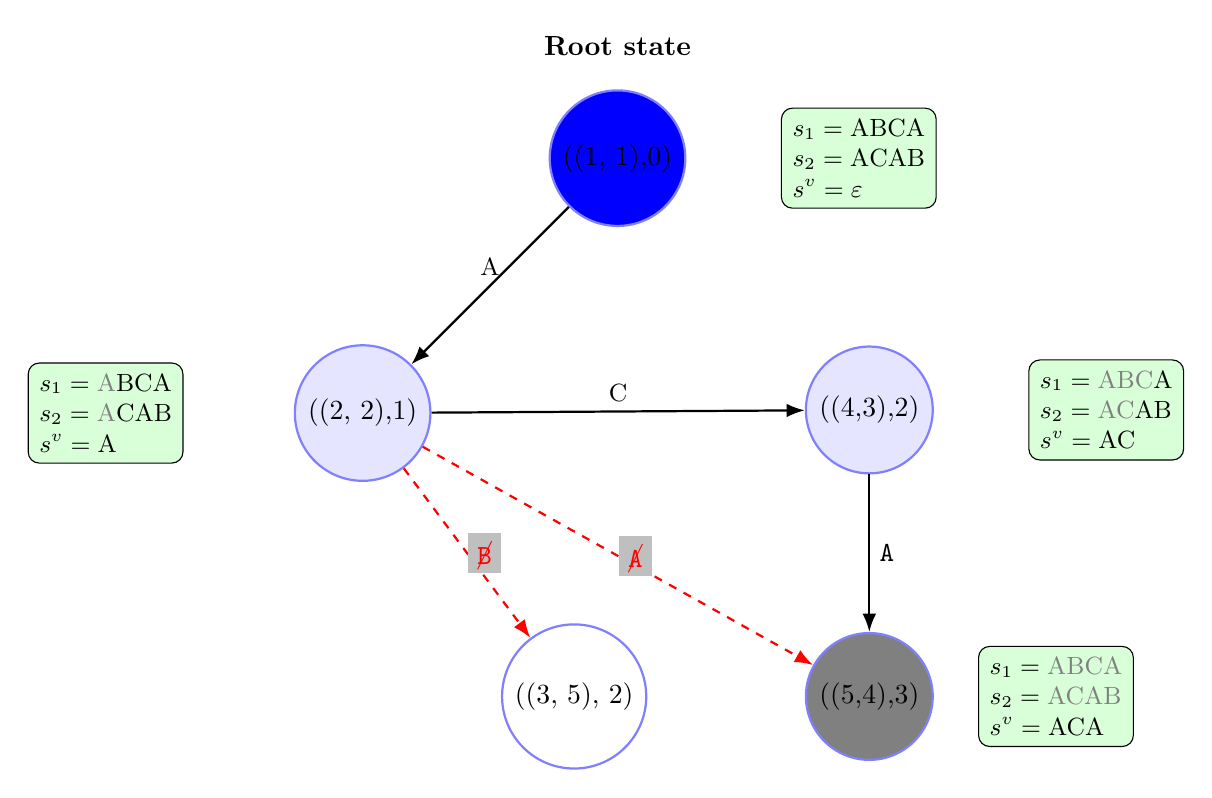
\begin{tikzpicture}[
   state/.style={circle, draw=blue!50, fill=blue!10, thick, minimum size=8mm},
   edge/.style={-Latex, thick},
   node distance=2cm and 2cm
   ]
   
   % Čvorovi
   \node[state, fill=blue] (s0) {((1, 1),0)};
   \node[state, below left=of s0] (s1) {((2, 2),1)};
   \node[state, below right=of s0] (s2) {((4,3),2)};
   %\node[state, below=of s2] (s3) {(4,3)};
   \node[state, below=of s2, fill=gray] (s4) {((5,4),3)}; % krajnje, ali ne koristi se ovde
   \node[state, left=of s4, fill=white] (s5) {((3, 5), 2)}; % krajnje, ali ne koristi se ovde
   
   % Right of root ((1,1),0)
   \node[box, right=12mm of s0] (b0) {
   $s_1=\text{{A}BCA}$\\
   $s_2=\text{{A}CAB}$\\
   $s^v=\varepsilon$
   };
   
   % Left of ((2,2),1)
   \node[box, left=14mm of s1] (b1) {
   $s_1=\text{\textcolor{gray}{A}BCA}$\\
   $s_2=\text{\textcolor{gray}{A}CAB}$\\
   $s^v=\text{A}$
   };
   
   % Right of ((4,3),2)
   \node[box, right=12mm of s2] (b2) {
   $s_1=\text{\textcolor{gray}{ABC}A}$\\
   $s_2=\text{\textcolor{gray}{AC}AB}$\\
   $s^v=\text{AC}$
   };
   
   % Right of ((5,4),3)
   \node[box, right=42mm of s5] (b3) {
   $s_1=\text{\textcolor{gray}{ABCA}}$\\
   $s_2=\text{\textcolor{gray}{ACAB}}$\\
   $s^v=\text{ACA}$
   };
   
 
   
   % Grane (samo validne poklapanja)
   \draw[edge] (s0) -- node[above] {\small A} (s1);
   %\draw[edge] (s0) -- node[above] {\small A} (s2);
   \draw[edge] (s1) -- node[above] {\small C} (s2);
   %\draw[edge] (s2) -- node[right] {\small A} (s3);
   %\draw[edge] (s3) -- node[right] {\texttt{A}} (s4);
   \draw[edge,  scale=2.2, dashed, red] (s1) -- node[right, fill=lightgray] {$\cancel{\texttt{B}}$} (s5);
   
    \draw[edge,  scale=2.2, dashed, red] (s1) -- node[right, fill=lightgray] {$\cancel{\texttt{A}}$} (s4);
   % Oznake
   \node[above=0.3cm of s0] {\textbf{Root state}};
   %\node[below=1.5cm of s3] {\small \textbf{Krajnje stanje}};
   \draw[edge] (s2) -- node[right] {\texttt{A}} (s4);
   
   \end{tikzpicture}}
   
   \caption{State space graph $Space(r=((1, 1), 0))$ for MVGLCSP between the sequences \texttt{ABCA} and  \texttt{ACAB}, assuming $G_1=G_2=1$.   % \fxnote{Add VGLCS example}
   }
   
   \label{fig:vgcs-grafstanja}
   \end{figure}
   
\end{frame}


\begin{frame}{An issue with the root-state-space formulation: example}

   \begin{itemize}
   \item The VGLCSP may exhibit multiple, potentially exponentially many, \emph{disconnected root components} in its complete state space.
   \item  If started from $(1, 1)$, it fails to reach    optimal solutions.     \end{itemize}
   \begin{example}
   		$
   		S = \{ s_1 = \texttt{ATGG\fbox{A}AA},\; s_2 = \texttt{ATCC\fbox{A}AA} \},
   		$
   		with gap constraints $G_{s_1} = G_{s_2} = 1$. In this instance, any state with position vector $\mathbf{p}^L = (5,5)$ cannot be reached  from the initial state $((1,1),0)$ by standard direct transitions. 

  \end{example} \vspace{0.5cm}
  
   \textbf{Consequence}: $((5, 5), 0) \not \in Space((1, 1))$  $\Rightarrow$  
   \textcolor{blue}{The optimal common subsequence \texttt{AAA} is unreachable.} %from the basic root $((1,1),0)$,  therefore missed by traditional search strategies.
   
\end{frame}

\begin{frame}{Iterative multi-source beam search (IMSBS) strategy}
      
      \begin{itemize}
      		\item \textbf{Full state space} of a VGLCSP instance: $\bigcup_{v \in \mathcal{R}} \mathrm{Space}(\mathbf{p}^{L, v})$, with $\mathcal{R}$ all root states %, i.e., states defined by position vectors (matches) $\mathbf{p}^{L,q}$ 
      		\item Explicitly enumerating all root states computationally prohibitive (requiring $O(n^m)$ time) \vspace{0.3cm}
      		\item \textbf{IMSBS} (idea):
      		\begin{itemize}
      		    \item Based on \textbf{beam search}: limited breadth-first-search (BFS) strategy (for exploring \emph{Space(r)})
      		    
      		    \item dynamically explore multiple promising regions of the state space: move from one rooted subgraph to another one 
      		    \item \textbf{iteratively identifies and expands} a set of \textcolor{red}{promising} candidate root states
      		\end{itemize}
      \end{itemize}  
\end{frame}

\begin{frame}{Components and characteristics of IMSBS}
     
     
     \begin{itemize}
     	\item $\mathcal{R}$: a global set of root-node candidates, dynamically updated over iterations
     	\item \textbf{Beam search} (backward): not all candidate nodes from $\mathcal{R}$ are root nodes
     	\begin{itemize}
     		\item \textcolor{blue}{\textbf{refine}} them by performing the \textcolor{blue}{\textbf{backward}} approximate passes from candidate-root nodes to effectively reach distant (real) and promising root node in the state space
     	\end{itemize}
     	\item \textcolor{blue}{\textbf{Beam search}} (forward): \textcolor{red}{intensification} in the chosen root-space \emph{Space(p)}: seek for high-quality (complete) solutions in the corresponding search sub-regions
     	\item \textcolor{red}{diversification}:  during each BS (forward), the complete nodes  are expanded in all possible ways (gaps ignored) to generate candidates for roots (distant from the current region)
     \end{itemize}

\end{frame}

\begin{frame}{Working example}
	 TODO: draw some plots regarding the workflow of the approach
	 
 
\end{frame}

\begin{frame}{The core advantages of the IMSBS approach}
 
     \begin{itemize}
     	\item Balance between complete beam search execution (local exploration of promising paths) and the generation of new source nodes (\textbf{global coverage} of the search space)
     	\item Preventing from direct suboptimal solutions reduced by executing backward beam search procedure (\textbf{refinement})
     \end{itemize}
      
\end{frame}

\begin{frame}{Heuristic guidances in BS}
    
    Three LCS heuristic guidances used:
        \begin{itemize}
       	    \item  \textit{``Look-ahead'' for the remaining length:}
    	    \begin{equation}
    		    \textrm{UB}_1(\mathbf{v}) = l^v + \min_{i = 1, \ldots, m} \left( |s_i| - p_i^v + 1 \right)
        	\end{equation}
    	  	\item  \textit{Character Frequency Alignment:}
    	   \begin{equation}
    	   	\textrm{UB}_2(\mathbf{v}) =  l^v + \sum_{\sigma \in \Sigma} 
    	   	\min\left(  |s_1[p_1^v, |s_1|]|_{\sigma}, \ldots, |s_m[p_m^v, |s_m|]|_{\sigma} \right)
    	   \end{equation}
    	   \item \textit{A probability-based heuristic} guidance by the pre-processed matrices of probabilities (Mousavi and Tabataba~(2012)). These probabilities approximate the probability for the event that a sequence $s$ of length $k$ is a subsequence of a (random) sequence of length $n$ %over an alphabet $\Sigma$.
    \end{itemize}
\end{frame}

\begin{frame}{Experimental Evaluation}
	TODO
\end{frame}

\end{document}
